% fig11_tbr_compare.tex — TBR: pool run vs adapter-embed vs EU-DEMO HCLL band.
% Compiled by the paper Makefile via `make figures` (pdflatex on the snippet).
%
% Data provenance (NO fabrication; commons @D g3) — Appendix E (app:tbr):
%   pool run     (transport-less-stub -> real OpenMC run) = 1.3197 +/- 0.0005
%   adapter-embed (transport in .hexa adapter, PR #1078)  = 1.3222 +/- 0.0004
%     (registered verify atom openmc_tbr_pb157li = 1.3222, SUPPORTED-NUMERICAL)
%   EU-DEMO HCLL self-sufficiency target band ~1.1-1.3 (Fischer et al. 2019,
%     fischer2019eudemoTBR) -- shaded reference band.
%   Self-sufficiency floor TBR = 1.0 (gate-(f) PASS criterion).
%   y-axis zoomed to 0.95-1.40 so the +-0.0005/0.0004 MC error bars are visible.
%
% Manual single-shot compile (debug):
%   pdflatex -interaction=nonstopmode -halt-on-error fig11_tbr_compare.tex
\documentclass[border=4pt]{standalone}
\usepackage{tikz}
\usetikzlibrary{calc}
\usepackage{pgfplots}
\pgfplotsset{compat=1.18}
\begin{document}
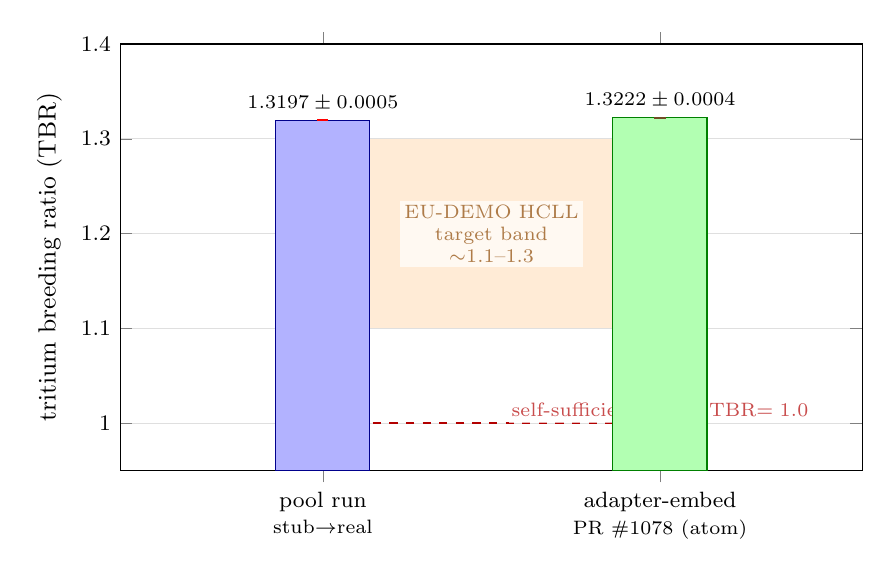
\begin{tikzpicture}
\begin{axis}[
  width=11cm, height=7cm,
  ybar,
  bar width=34pt,
  ymin=0.95, ymax=1.40,
  ylabel={tritium breeding ratio (TBR)},
  symbolic x coords={pool, embed},
  xtick={pool, embed},
  xticklabels={%
    \shortstack{pool run\\\scriptsize stub$\to$real},
    \shortstack{adapter-embed\\\scriptsize PR \#1078 (atom)}},
  x tick label style={font=\footnotesize,align=center},
  tick label style={font=\footnotesize},
  label style={font=\small},
  ymajorgrids,
  grid style={gray!25},
  enlarge x limits=0.6,
  clip=false,
]
% EU-DEMO HCLL target band ~1.1-1.3 (shaded) -- drawn as a filled rectangle
\fill[orange!16] (axis cs:pool,1.1) rectangle (axis cs:embed,1.3);
\node[font=\scriptsize,text=orange!55!black,anchor=center,fill=white,fill opacity=0.7,inner sep=1.5pt,align=center]
  at ($(axis cs:pool,1.20)!0.5!(axis cs:embed,1.20)$) {EU-DEMO HCLL\\target band\\$\sim$1.1--1.3};
% self-sufficiency floor TBR = 1.0
\addplot[draw=red!70!black,dashed,thick,sharp plot,update limits=false] coordinates {
  (pool,1.0) (embed,1.0)
};
\node[font=\scriptsize,text=red!70!black,anchor=south,fill=white,fill opacity=0.7,inner sep=1pt]
  at (axis cs:embed,1.0) {self-sufficiency floor TBR$=1.0$};
% the two TBR bars with error bars
\addplot+[draw=blue!55!black,fill=blue!30,bar shift=0pt,
  error bars/.cd, y dir=both, y explicit] coordinates {
  (pool,1.3197) +- (0,0.0005)
};
\addplot+[draw=green!50!black,fill=green!30,bar shift=0pt,
  error bars/.cd, y dir=both, y explicit] coordinates {
  (embed,1.3222) +- (0,0.0004)
};
% value annotations
\node[font=\scriptsize,anchor=south] at (axis cs:pool,1.3197)
  {$1.3197\pm0.0005$};
\node[font=\scriptsize,anchor=south] at (axis cs:embed,1.3222)
  {$1.3222\pm0.0004$};
\end{axis}
\end{tikzpicture}
\end{document}
